\documentclass[12pt,letterpaper]{article}
\usepackage{graphicx,textcomp}
\usepackage{natbib}
\usepackage{setspace}
\usepackage{fullpage}
\usepackage{color}
\usepackage[reqno]{amsmath}
\usepackage{amsthm}
\usepackage{fancyvrb}
\usepackage{amssymb,enumerate}
\usepackage[all]{xy}
\usepackage{endnotes}
\usepackage{lscape}
\newtheorem{com}{Comment}
\usepackage{float}
\usepackage{hyperref}
\newtheorem{lem} {Lemma}
\newtheorem{prop}{Proposition}
\newtheorem{thm}{Theorem}
\newtheorem{defn}{Definition}
\newtheorem{cor}{Corollary}
\newtheorem{obs}{Observation}
\usepackage[compact]{titlesec}
\usepackage{dcolumn}
\usepackage{tikz}
\usetikzlibrary{arrows}
\usepackage{multirow}
\usepackage{subcaption}
\usepackage{xcolor}
\newcolumntype{.}{D{.}{.}{-1}}
\newcolumntype{d}[1]{D{.}{.}{#1}}
\definecolor{light-gray}{gray}{0.65}
\usepackage{url}
\usepackage{listings}
\usepackage{color}
\usepackage{comment}

\definecolor{codegreen}{rgb}{0,0.6,0}
\definecolor{codegray}{rgb}{0.5,0.5,0.5}
\definecolor{codepurple}{rgb}{0.58,0,0.82}
\definecolor{backcolour}{rgb}{0.95,0.95,0.92}

\lstdefinestyle{mystyle}{
	backgroundcolor=\color{backcolour},   
	commentstyle=\color{codegreen},
	keywordstyle=\color{magenta},
	numberstyle=\tiny\color{codegray},
	stringstyle=\color{codepurple},
	basicstyle=\footnotesize,
	breakatwhitespace=false,         
	breaklines=true,                 
	captionpos=b,                    
	keepspaces=true,                 
	numbers=left,                    
	numbersep=5pt,                  
	showspaces=false,                
	showstringspaces=false,
	showtabs=false,                  
	tabsize=2
}
\lstset{style=mystyle}
\newcommand{\Sref}[1]{Section~\ref{#1}}

\title{ PS Response}
\date{Victor Gomez}
\author{Applied Stats/Quant Methods 1}

\begin{document}
	\maketitle
	

\section*{Problem 1 }

\textit{Preliminary code}\\

\vspace{.25cm}

\noindent  Here is first a succint presentation of dataset.  This one used is a sample $y$ of 25 IQ values of students.\\
Loaded as follows:

\lstinputlisting[language=R, firstline=41, lastline=41]{PS01_Victor_Gomez.R}  

\noindent  Which can be summarised with

\lstinputlisting[language=R, firstline=42, lastline=42]{PS01_Victor_Gomez.R}  
\begin{verbatim}
   Min. 1st Qu.  Median    Mean 3rd Qu.    Max. 
  69.00   89.00   98.00   98.44  110.00  126.00
\end{verbatim}

\vspace{.5cm}

\subsection*{Question 1}

We assume that the sample follow a Sutend distribution of $\# y -1$ degrees of freedom, since its size is small ($\lesssim 30 $).
Therefore, the confidence interval CI at 90\% confidence (or at risk $\alpha :=0.1$) is 
\begin{align*}
	CI_{90\%} = [\bar{y} - T(0.95).se(y) , \bar{y} +  T(0.95).se(y) ]
\end{align*}
where $se$ states for standard error, and \\
$T$ is the Student  cumulative distribution function

Which leads to the following code:

\lstinputlisting[language=R, firstline=47, lastline=56]{PS01_Victor_Gomez.R}  

Which result is :

\begin{verbatim}
	[1]  93.95993 102.92007
\end{verbatim}
for lower and upper bound respectively. I.e. $CI_{90\%} = [93.95993, 102.92007]$

\vspace{.5cm}

\subsection*{Question 2}

We consider Hypothesis $ \mathcal{H}_0$ as  "Average student IQ is lower or equal than the average IQ score among all the schools int he country." \\
We denote $\mu_{general}$ the mean of general population ( $\mu_{general} = 100$ ) and $\mu_{student}$ the IQ mean of the students.\\
I.e. 
\begin{align*}
	 \mathcal{H}_0 := \{ \mu_{general} \geqslant \mu_{students} \}
\end{align*}

So, the test statistic $T$ is

\begin{align*}
	 T := \frac{\bar{y}-\mu_{general}}{\sigma_y / \sqrt{n}}
\end{align*}
where $\sigma_y$ is the standard deviation of the sample $y$ and $\sqrt{n}:= \# y $. 
\vspace{.25cm}
We apply a one-sidded T-test to this hypothesis, with risk $\alpha :=5\%$

\lstinputlisting[language=R, firstline=65, lastline=68]{PS01_Victor_Gomez.R}  

\begin{verbatim}
> test

	One Sample t-test

data:  y
t = -0.59574, df = 24, p-value = 0.7215
alternative hypothesis: true mean is greater than 100
95 percent confidence interval:
 93.95993      Inf
sample estimates:
mean of x 
    98.44 

> test$p.value
[1] 0.7215383
\end{verbatim}


I.e the p-value is $0.7215383$.  $\mathcal{H}_0$ is not rejected.

%\textit{Note:  In fact, we consider here that mean of the sample is the true mean of all students.}

\section*{Problem 2}

\subsection*{Question 1}

\begin{figure}[h!]\centering
	\caption{\footnotesize Pair plot between $Y,X1,X2,X3$ }
	\label{fig:plot_0}
	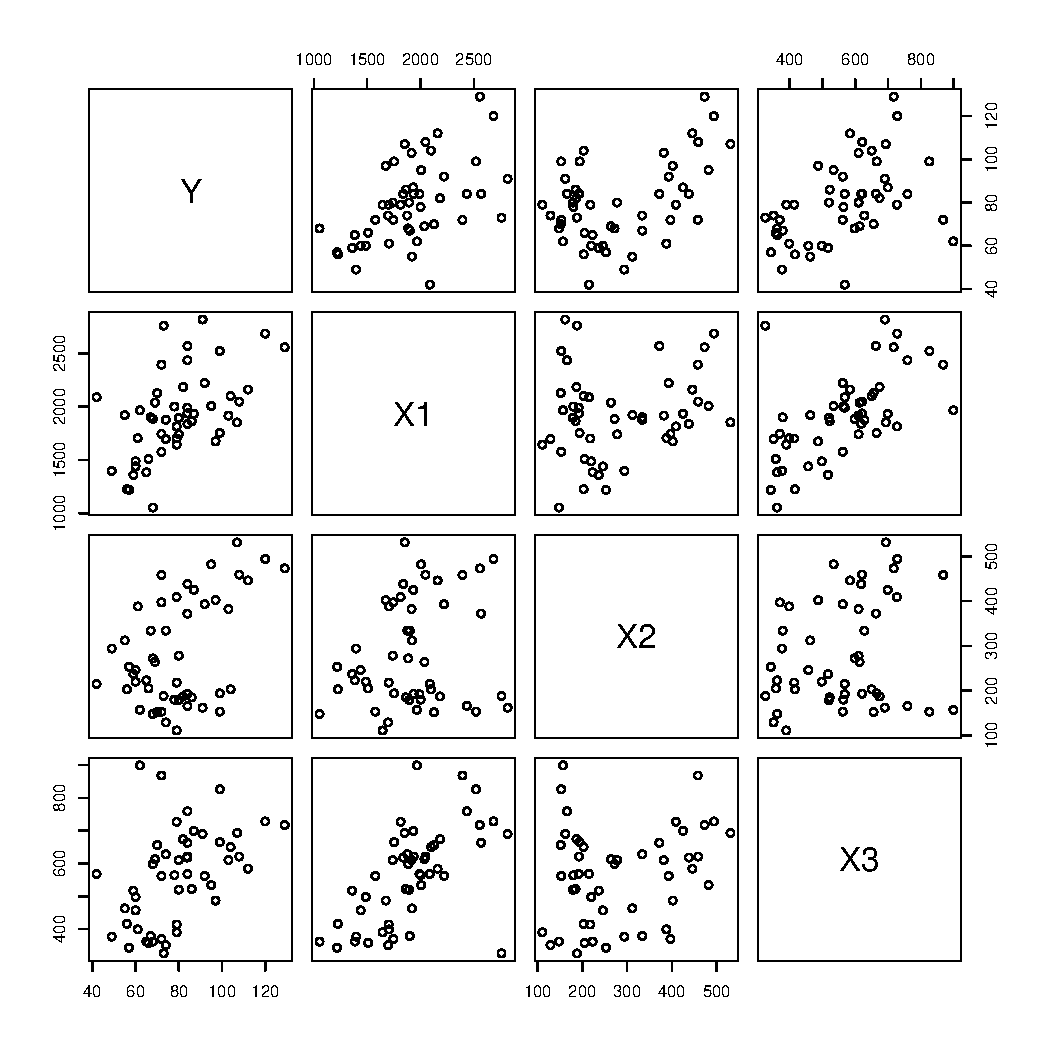
\includegraphics[width=.85\textwidth]{pairs.pdf}
\end{figure}

The plot above shows the bivariate relationship between $Y,X1,X2,X3$ variables.  Relationships between $X1$ and $X2$, and $X2$ and $X3$ seem aleatory. However, $X1$ and $X3$ seem to have a linear relation. \\
Then $Y$ seem to have some positive correlation (in  	Spearman's correlation coefficient sens, i.e. here, linearity is not obvious)  with $X1$  $X3$, a linear relationship with $X1$, and $Y$-$X2$ relationship seems parabolic. For further analysis, a covariance matrix would be appropriated (for linear relationships only).

\subsection*{Question 2}

\begin{figure}[h!]\centering
	\caption{\footnotesize Relationship between $Y$ and Region }
	\label{fig:plot_1}
	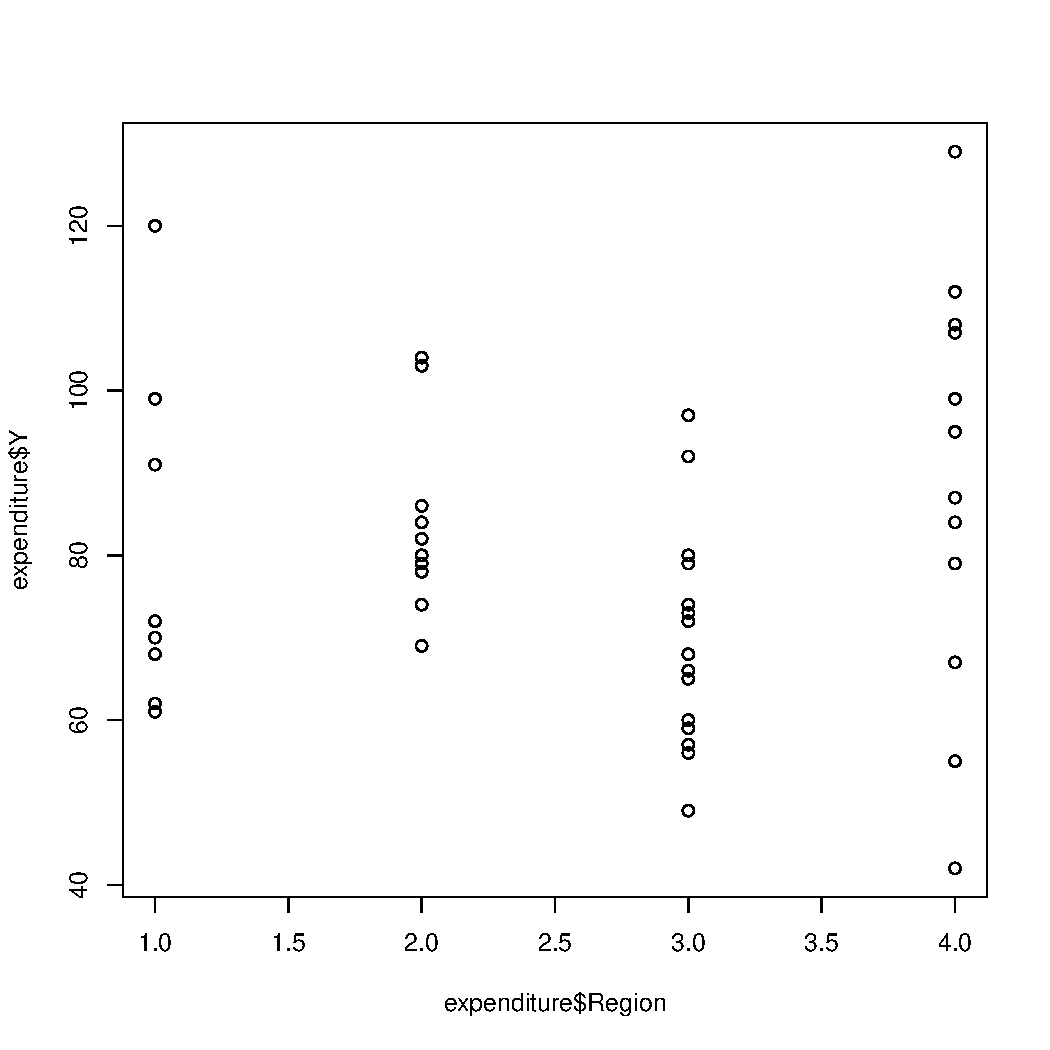
\includegraphics[width=.85\textwidth]{regions.pdf}
\end{figure}

\begin{figure}[h!]\centering
	\caption{\footnotesize Boxplot of $Y$ according to $Region$ }
	\label{fig:plot_2}
	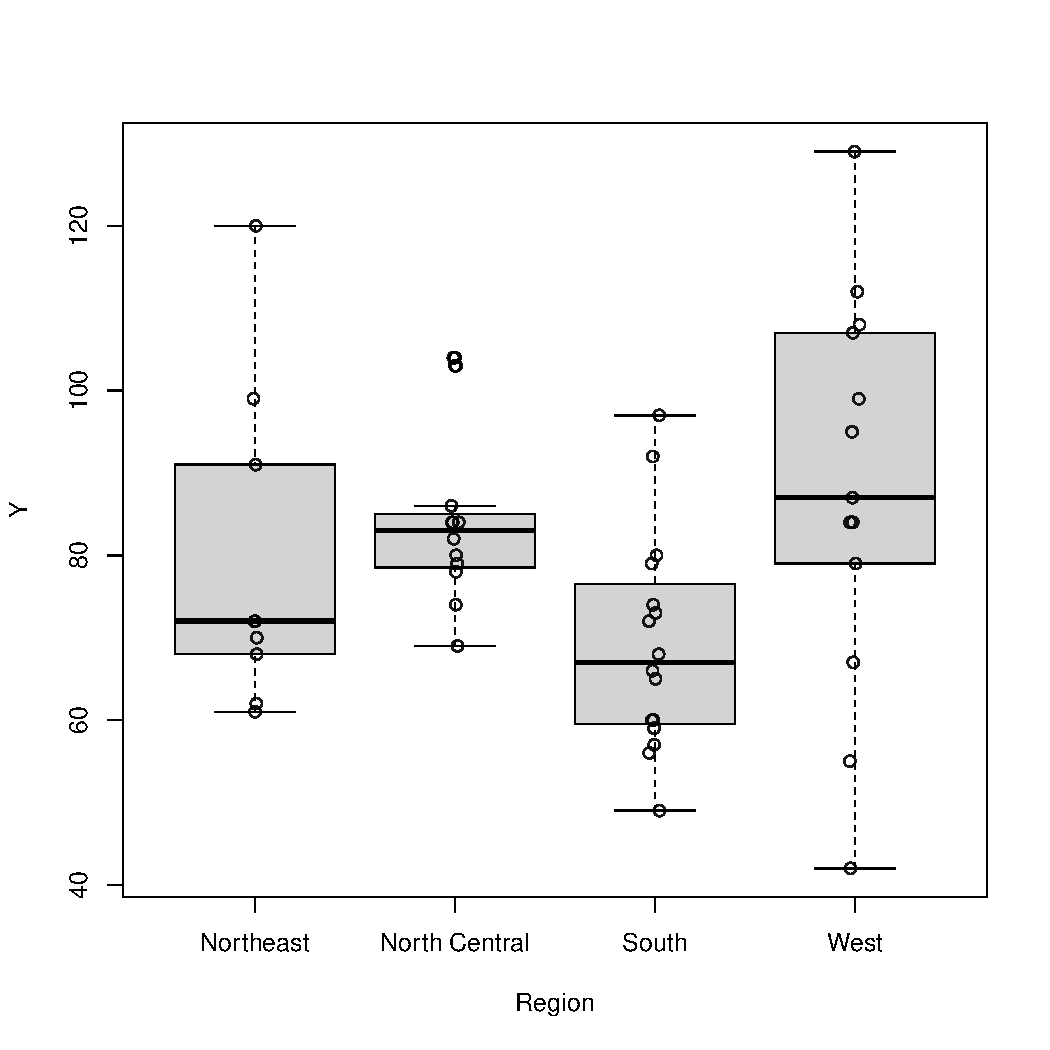
\includegraphics[width=.85\textwidth]{regions_boxplot.pdf}
\end{figure}

Considering the two graphs above, the region with, in average, the highest per capita expenditure on housing assistance is $West$. Indeed, even if the first graph is not easily interpretable, the box plot that $West$ has the highest median (~90\$/capita) more or less centered between min (~45\$/capita) and max (~110\$/capita) were at the lower third between  the$ 1^{st}$ and the $3^{rd}$ quantile. Thus, average for $West$ region should be higher than the median. On the other hand, the $3^{rd}$ quantile of $North central$  and $South$ are below the median of $West$ region and their maxima are under the $3^{rd}$ quantile of $West$. This leads to consider that their respective means should be under the mean of $West$ region. 
Finally, $Northeast$ has more dispersion, while its median is below $1^{rst}$ quantile of $West$. Its $3^{rd}$ quantile is more or less equal to $West$'s median and its maximum is below $West$'s maximum. I.e. ,  mean of $Northeast$'s region is below $West$ average.
\\
To confirm this visual analysis, it suffice to calculate the actual means of each region sample.

\subsection*{Question 3}

The following graph is a reproduction of one of the plot of  Fig.\ref{fig:plot_0} where are added $Region$ repartition by colours.

\begin{figure}[h!]\centering
	\caption{\footnotesize Relationship between $Y$ and $X1$ showing $Regions$ }
	\label{fig:plot_3}
	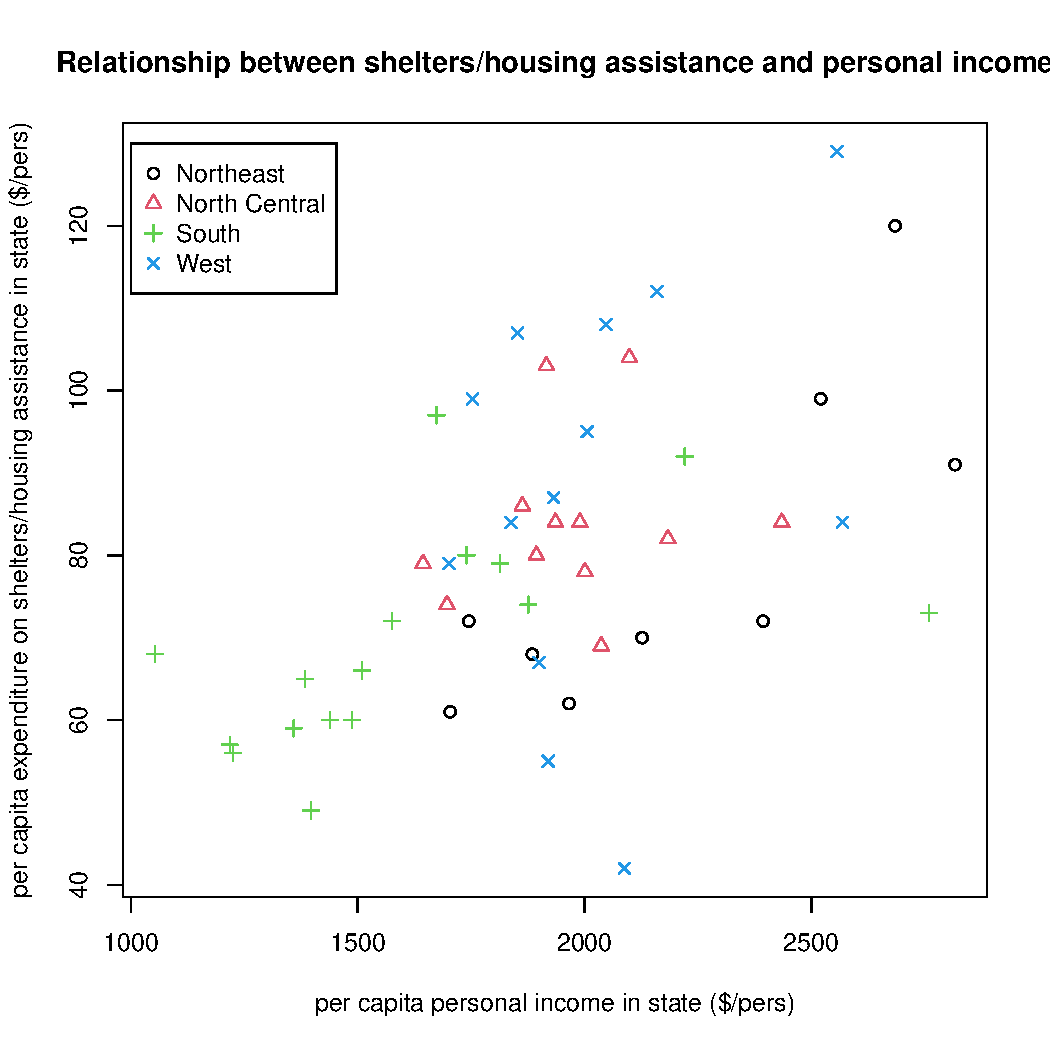
\includegraphics[width=.85\textwidth]{YX1Region.pdf}
\end{figure}

The Fig.\ref{fig:plot_3} shows that $South$ region's people have mainly lower income than others (mainly between  1200 and 1600 \$/pers.) and use generally give between 50 and 70\$/pers. for shelters or housing assistance. \\
$North Central$ follows the smae pattern of a centered group , but with higher incomes and higher expenditure (respectively between 1700 and 2200\$/pers. and 70 and 100\$/pers.). \\
At the contrary, the expenditure givien by $West$ region's sample seems not to be correlated to $X1$ variable, since the main income is between 1700 and 2100\$/pers. were as expenditure are spread from 60\$/pers. to 110\$/pers.  \\
Concerning $Northeast$ region, it is difficult to give any comment, since sample values are scarce and scattered. \\

In order to be compleate, it has to be mentioned that the samples for each region are little, thus, intervals given above are unprecise and have to be considered as rough approximations.

To conclude regional analysis, $South$ and $North Central$ region seem to from punctual clusters, the former below the latter for two edges. In addition, $West$ expenditure seems to be indifferent to personal income, and it is not possible to conclude concerning $Northeast$ region.

Finally, concerning the general relation between per capita expenditure on shelters and housing and per capita personal income, it might appear a linear relation, without homoscedasticity, i.e. with a growing dispersion along per capita personal income variable.

\end{document}


\begin{comment}
\noindent You can also save figures in R, and place them in your answers that you're writing in your .tex file. First, you need to make sure your path/file name is correct, then you'll save your work when your in R (see code below).

\lstinputlisting[language=R, firstline=52, lastline=55]{PS01_Victor_Gomez.R}  
\vspace{.25cm}
\noindent With our figure saved, we just need to render it in our .tex file, which we can do using the \texttt{figure} environment:

\begin{verbatim}
	\begin{figure}[h!]\centering
		\caption{\footnotesize Example from base plot in R.}
		\label{fig:plot_1}
		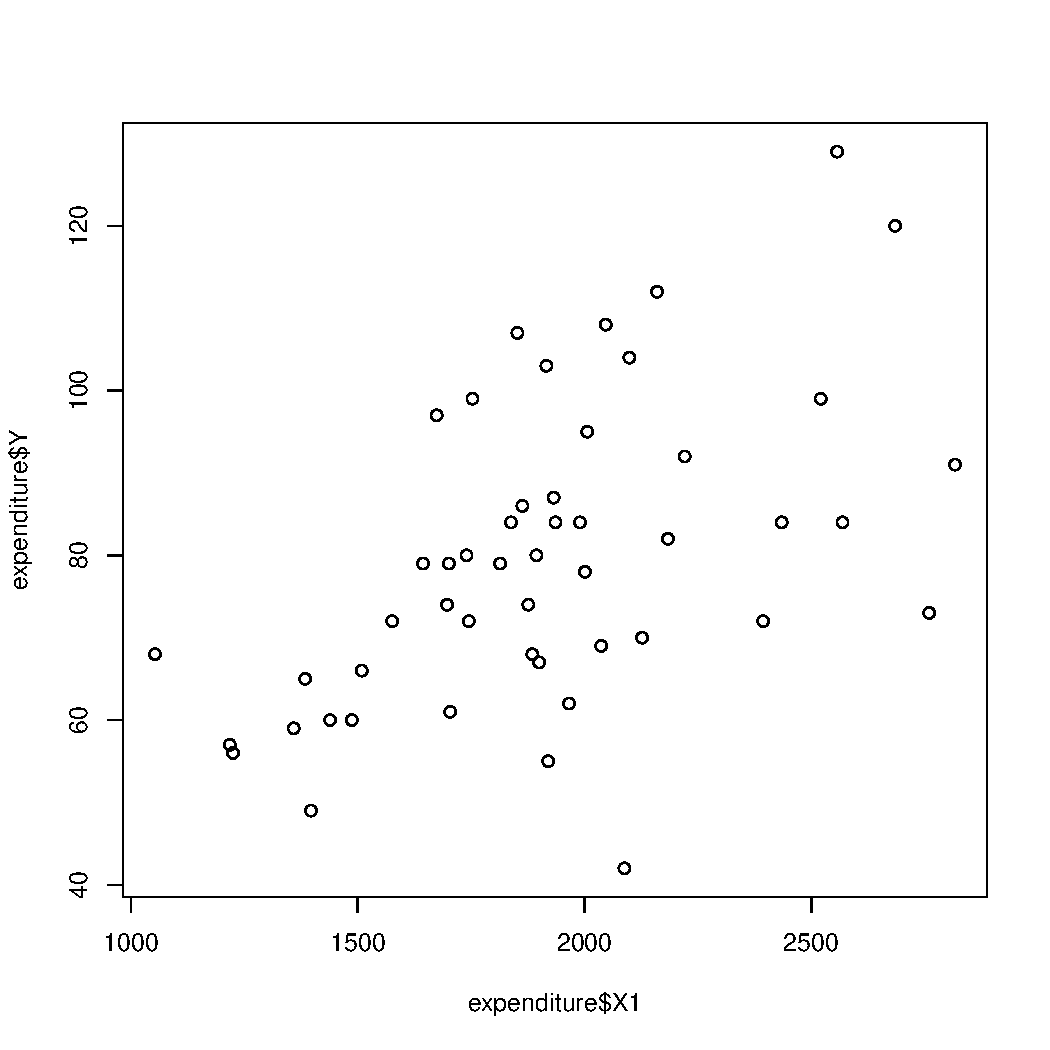
\includegraphics[width=.85\textwidth]{plot_example.pdf}
	\end{figure}
\end{verbatim}

\begin{figure}[h!]\centering
	\caption{\footnotesize Example from base plot in R.}
	\label{fig:plot_1}
	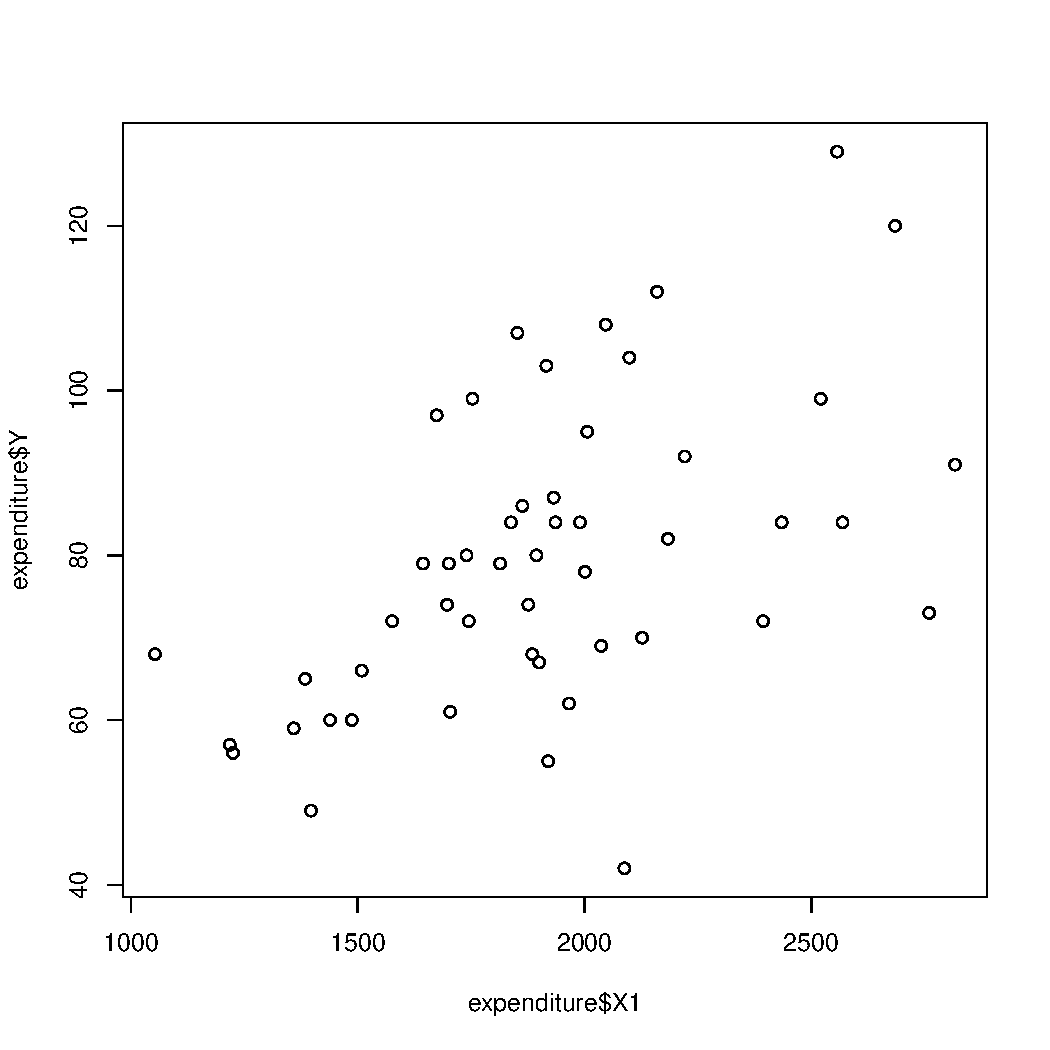
\includegraphics[width=.75\textwidth]{plot_example.pdf}
\end{figure}

\noindent Finally can also save tables in R, and place them in your answers in your .tex file, just like you would a figure. You will essentially dump and save the information in a new file, and then read that file in through Latex.

\lstinputlisting[language=R, firstline=57, lastline=66]{PS01_Victor_Gomez.R}  

\noindent That's great, you saved your table in a new file in the same folder as your .tex and .R files. Now, let's read in our saved table using \texttt{$\backslash$input{regression\_output1.tex}}, which will result in:


% Table created by stargazer v.5.2.3 by Marek Hlavac, Social Policy Institute. E-mail: marek.hlavac at gmail.com

\begin{table}[!htbp] \centering 
  \caption{} 
  \label{} 
\begin{tabular}{@{\extracolsep{5pt}}lc} 
\\[-1.8ex]\hline 
\hline \\[-1.8ex] 
 & \multicolumn{1}{c}{\textit{Dependent variable:}} \\ 
\cline{2-2} 
\\[-1.8ex] & Y \\ 
\hline \\[-1.8ex] 
 X1 & 0.025$^{***}$ \\ 
  & (0.006) \\ 
  & \\ 
 Constant & 32.546$^{***}$ \\ 
  & (11.034) \\ 
  & \\ 
\hline \\[-1.8ex] 
Observations & 50 \\ 
R$^{2}$ & 0.283 \\ 
Adjusted R$^{2}$ & 0.268 \\ 
Residual Std. Error & 15.836 (df = 48) \\ 
F Statistic & 18.920$^{***}$ (df = 1; 48) \\ 
\hline 
\hline \\[-1.8ex] 
\textit{Note:}  & \multicolumn{1}{r}{$^{*}$p$<$0.1; $^{**}$p$<$0.05; $^{***}$p$<$0.01} \\ 
\end{tabular} 
\end{table}  

% Table created by stargazer v.5.2.3 by Marek Hlavac, Social Policy Institute. E-mail: marek.hlavac at gmail.com
% Date and time: mer., sept. 25, 2024 - 11:20:54
\begin{table}[!htbp] \centering 
  \caption{} 
  \label{} 
\begin{tabular}{@{\extracolsep{5pt}}lc} 
\\[-1.8ex]\hline 
\hline \\[-1.8ex] 
 & \multicolumn{1}{c}{\textit{Dependent variable:}} \\ 
\cline{2-2} 
\\[-1.8ex] & Y \\ 
\hline \\[-1.8ex] 
 X1 & 0.025$^{***}$ \\ 
  & (0.006) \\ 
  & \\ 
 Constant & 32.546$^{***}$ \\ 
  & (11.034) \\ 
  & \\ 
\hline \\[-1.8ex] 
Observations & 50 \\ 
R$^{2}$ & 0.283 \\ 
Adjusted R$^{2}$ & 0.268 \\ 
Residual Std. Error & 15.836 (df = 48) \\ 
F Statistic & 18.920$^{***}$ (df = 1; 48) \\ 
\hline 
\hline \\[-1.8ex] 
\textit{Note:}  & \multicolumn{1}{r}{$^{*}$p$<$0.1; $^{**}$p$<$0.05; $^{***}$p$<$0.01} \\ 
\end{tabular} 
\end{table}  

% Table created by stargazer v.5.2.3 by Marek Hlavac, Social Policy Institute. E-mail: marek.hlavac at gmail.com
% Date and time: jeu., sept. 26, 2024 - 13:46:28
\begin{table}[!htbp] \centering 
  \caption{} 
  \label{} 
\begin{tabular}{@{\extracolsep{5pt}}lc} 
\\[-1.8ex]\hline 
\hline \\[-1.8ex] 
 & \multicolumn{1}{c}{\textit{Dependent variable:}} \\ 
\cline{2-2} 
\\[-1.8ex] & Y \\ 
\hline \\[-1.8ex] 
 X1 & 0.025$^{***}$ \\ 
  & (0.006) \\ 
  & \\ 
 Constant & 32.546$^{***}$ \\ 
  & (11.034) \\ 
  & \\ 
\hline \\[-1.8ex] 
Observations & 50 \\ 
R$^{2}$ & 0.283 \\ 
Adjusted R$^{2}$ & 0.268 \\ 
Residual Std. Error & 15.836 (df = 48) \\ 
F Statistic & 18.920$^{***}$ (df = 1; 48) \\ 
\hline 
\hline \\[-1.8ex] 
\textit{Note:}  & \multicolumn{1}{r}{$^{*}$p$<$0.1; $^{**}$p$<$0.05; $^{***}$p$<$0.01} \\ 
\end{tabular} 
\end{table}  


\noindent Or, you can paste the code you get from \texttt{stargazer} in R into the \texttt{verbatim} environment in Latex. This is more labor intensive, but produces the same results.
\end{comment}